\documentclass{article}

\usepackage[brazil]{babel}

\usepackage[letterpaper,top=2cm,bottom=2cm,left=3cm,right=3cm,marginparwidth=1.75cm]{geometry}
\usepackage{amsmath}
\usepackage{tabularx}
\usepackage{graphicx}
\usepackage[colorlinks=true, allcolors=blue]{hyperref}
\usepackage{caption}
\usepackage{float}

\sloppy

\begin{document}

\begin{titlepage}
	\begin{center}
		{\large Universidade Federal de Minas Gerais}\\[0.2cm]
		{\large Instituto de Ciências Exatas}\\[0.2cm]
		{\large Departamento de Ciência da Computação}\\[0.2cm]
		{\large Projeto Final de Aprendizado Descritivo}\\[5.1cm]
		{\large \bf Mineração de Dados de Eventos em Futebol}\\[5.1cm]
	\end{center}
	{\large Alunos: Luís Felipe Ramos Ferreira, Igor Lacerda Faria da
	Silva,
	Matheus Tiago Pimenta de Souza}\\[0.7cm]
	{\large Professor: Renato Vimieiro}\\[5.1cm]
	\begin{center}
		{\large Belo Horizonte - Minas Gerais}\\[0.2cm]
		{\large 2024}
	\end{center}
\end{titlepage}

\newpage
\renewcommand{\contentsname}{Sumário}
\tableofcontents
\newpage

\title{Mineração de Dados de Evento em Futebol}
\author{Luís Felipe Ramos Ferreira \\  Igor Lacerda iFaria da Silva \\ Matheus
	Tiago Pimenta de Souza}

\maketitle

\section{Introdução}

O uso de ciência de dados e estatística para analisar esportes é algo que vem
crescendo cada vez mais nos últimos anos. Em
particular, o futebol tem sido um desses
esportes \cite{takvorian2021beautiful}. Diversas empresas que atuam na
área surgem a cada dia, e os times de futebol, no Brasil e no resto do
mundo, estão investindo em seus departamentos de dados e estatística.

Nesse sentido, este trabalho propõe estudar e compreender melhor como funciona
o uso de análises estatísticas no futebol, dado o interesse do público geral pelo esporte,
e, para isso, propomos a aplicação de algoritmos de mineração de dados em
dados futebolísticos, sendo eles dados de súmula e dados de eventos das partidas, 
para compreender como as informações acerca do
jogo estão contidas dentro dos dados coletados e como isso pode ser utilizado a
favor das equipes.

Os dados de eventos, especialmente, costumam ser mais fáceis de lidar e mais
fáceis de acessar do que dados de \textit{tracking}, enquanto trazem muito mais
informações do que dados de súmula. Existem, atualmente, algumas bases
gratuitas de dados de evento de partidas, disponibilizadas por diferentes
empresas como \textit{Wyscout} e \textit{StasBomb}.

\subsection{Base de dados}

A principal base disponibilizada pela empresa \textit{Wyscout} foi usada como
base de dados. Ela contém dados de evento das 5 grandes ligas europeias na
temporada 17/18.

Cada empresa fornecedora de dados possui seu próprio formato de representação
dos dados de evento. De modo a facilitar a mesclagem entre as bases de dados
utilizadas, iremos converter os dados coletados para uma representação geral
proposta por pesquisadores denominada
\href{https://socceraction.readthedocs.io/en/latest/documentation/spadl/spadl.html}{SPADL}.
A SPADL é uma boa escolha por ser uma representação concisa e fácil de
utilizar. Ela é uma representação tabular de cada evento da partida, onde cada
linha possui 12 colunas. A tabela abaixo ilustra o esquema de representação de
um evento segundo o formato SPADL.

\begin{table}[H]
	\centering
	\begin{tabular}{|l|l|}
		\hline
		\textbf{Atributo} & \textbf{Descrição}
		\\
		\hline
		game\_id          & O ID do jogo no qual a ação foi realizada
		\\
		\hline
		period\_id        & O ID do período do jogo no qual a ação foi
		realizada
		\\
		\hline
		seconds           & O tempo de início da ação
		\\
		\hline
		player            & O jogador que realizou a ação
		\\
		\hline
		team              & O time do jogador
		\\
		\hline
		start\_x          & A localização x onde a ação começou
		\\
		\hline
		start\_y          & A localização y onde a ação começou
		\\
		\hline
		end\_x            & A localização x onde a ação terminou
		\\
		\hline
		end\_y            & A localização y onde a ação terminou
		\\
		\hline
		action\_type      & O tipo de ação (por exemplo, passe, chute,
		drible)
		\\
		\hline
		result            & O resultado da ação (por exemplo, sucesso
		ou falha)
		\\
		\hline
		bodypart          & A parte do corpo do jogador usada para a
		ação
		\\
		\hline
	\end{tabular}
	\caption{Descrição dos dados no formato SPADL}
	\label{tab:atributosSPADL}
\end{table}

\section{Implementação}

A linguagem escolhida para o desenvolvimento do trabalho foi
\href{https://www.python.org/}{\texttt{Python}} (versão 3.10.12), devida a seu
vasto ecossistema para ciência de dados e mineração de dados.

A manipulação dos dados foi feita com o uso de bibliotecas
de análise numérica como \href{https://numpy.org/}{\texttt{NumPy}} e
manipulação de \textit{dataframes} como
\href{https://pola.rs/}{\texttt{Polars}} e
\href{https://pandas.pydata.org/}{\texttt{Pandas}},
uma vez que se tratam de ferramentas extremamente completas que facilitaram o
desenvolvimento do projeto como um todo.

Para aplicar os algoritmos de descobertas de subgrupos, foi utilizado os pacote
\href{https://pysubgroup.readthedocs.io/en/latest/}{\texttt{pysubgroup}}, que fornecem 
uma aglomeração de algoritmos do estado da arte de descoberta de subgrupos em um formato simples 
e leve para serem utilizados. Também foi utilizada a implementação do algoritmo 
\href{https://github.com/HMProenca/SSDpp-numeric/tree/master}{\texttt{SSD++ para valores numéricos}},
um dos métodos mais recentes utilizado nos artigos 
\cite{proencca2021discovering}
e \cite{vagliano2023automated}.

falar dos pacotes de mineração de seq aqui

Para organizar o ambiente de desenvolvimento, que englobava vários pacotes
diferentes, foi utilizado o gerenciador de pacotes
\href{https://www.anaconda.com/}{\texttt{Anaconda}}, o que facilitou o trabalho
com os pacotes de ciência de dados citados. O projeto final foi salvo em um
\href{https://github.com/lframosferreira/projeto-ad}{\texttt{repositório}}
no GitHub para fácil versionamento e organização de código. As instruções de
como utilizar o que foi implementado estão descritas no \textit{README}
do repositório.

\section{Referencial Teórico}

No decorrer do trabalho, duas importantes métricas de análise ofensiva no
futebol serão utilizadas. Esta seção
aglomera os conhecimentos necessários sobre elas para a compreensão do projeto
e o como elas foram utilizadas.

\subsection{Gols Esperados (\textit{xG})}

Intuitivamente, existe a noção de que, quanto mais próximo um jogador está do
gol, mais chance ele tem de conseguir marcar um ponto para sua equipe. Uma
noção similar existe para o ângulo entre o gol e jogador: é mais difícil um
atacante acertar se ele está em uma das laterais. Na área de \textit{analytics}
de futebol, essa noção é formalizada através da métrica de \textit{expected
goals}, ou \textit{xG}. A ideia central é construir um modelo do que um jogador
médio faria em dado estado de jogo, que, além de incluir os fatores mencionados
anteriormente, pode ser mais (ou menos) extensivo.

A métrica de Gols Esperados captura um estado de jogo e retorna uma
probabilidade estimada de um jogador marcar. Ela pode ser vista como um
\textit{framework}, cujos detalhes de implementação são decididos pelo usuário.
Outros fatores considerados importantes são: parte do corpo associada à ação
(pé dominante ou não; de cabeça), origem da assistência (cruzamento, passe) e a
posição dos defensores. Para avaliar este último quesito, é necessário ter
dados de \textit{tracking}, o que limita consideravelmente sua adoção. Além disso,
mesmo questões como a liga em análise podem ser relevantes.

O uso do \textit{xG} é mais amplo do que se pode imaginar a princípio. Em um
primeiro momento, partidas podem ser analisadas: é possível avaliar se um time
fez mais ``pressão'' pela soma do seu \textit{xG} na partida. No entanto, como
com qualquer outro indicador, o \textit{xG} não define absolutamente o
resultado de um jogo, podendo um time aproveitar muito bem situações menos
favoráveis. Outra aplicação é avaliação de jogadores: se um jogador
consistentemente faz gols em situações desfavoráveis, isso é um grande indício
de que ele é jogador de destaque, ou age muito bem sob pressão. O \textit{xG}
também pode ser usado taticamente, para proporcionar melhorias no
posicionamento dos jogadores da \textit{defesa} e para embasar estratégias.

É comum usar modelos de regressão logística para aplicar o \textit{xG}, em que
se considera uma combinação dos fatores mencionados anteriormente. Essa
combinação não é necessariamente linear: considerar o quadrado da distância
pode ser valioso, por exemplo. Na prática, no entanto, qualquer modelo de
classificação binária pode ser usado. Um exemplo muito prevalente é o
\textit{xG} do \textit{Statsbomb}, que usa um \textit{XGBoost} e considera a
quantidade e a posição dos jogadores entre o gol e o jogador que faz o lance.

\subsection{Valuing Actions by Estimating Probabilities (VAEP)}

O \textit{xG} deixa a desejar em alguns aspectos. Principalmente pelo fato de
focar exclusivamente nas chances de se fazer gols, sem considerar outros
aspectos importantes do jogo. Por exemplo, existem passes que são cruciais para
uma equipe se aproximar do gol. É justamente para suprir a necessidade de
avaliar as ações dos jogadores de forma mais ampla que foi desenvolvido o VAEP
\cite{vaep}. O VAEP avalia cada ação do jogo em termos do quanto ela aumenta (ou
diminui) a chance de um time fazer (ou sofrer) um gol.

Com base no estado atual do jogo (placar, tempo restante, ações anteriores,
posição da bola, etc), o VAEP estima a chance de um time fazer ou sofrer um gol,
antes e após cada ação. Desse modo, é possível estimar a utilidade de uma ação
com base na diferença entre as mudanças de se fazer e de se sofrer um gol.
Formalizando, temos que, para um dado time $t$, uma ação $a_i$ e um estado de
jogo $S_i$:

\begin{equation}
	\Delta P_{score}(a_i,t) = P^k_{score}(S_i,t) - P^k_{score}(S_{i-1},t)
	\label{eq:vaep_scores}
\end{equation}

\begin{equation}
	\Delta P_{concede}(a_i,t) = P^k_{concede}(S_i,t) - P^k_{concede}(S_{i-1},t)
	\label{eq:vaep_concedes}
\end{equation}

\begin{equation}
	V_{\textrm{VAEP}}(a_i) = \Delta P_{score}(a_i,t) - \Delta P_{concede}(a_i,t) 
	\label{eq:vaep}
\end{equation}

Nas equações, $k$ é um parâmetro que indica quantas jogadas futuras estão sendo
consideradas para se avaliar a jogada atual. Assim, quando uma jogada aumenta
muito a chance de um gol acontecer, seu VAEP é um número positivo e, caso a
jogada ofereça mais risco do que recompensa, o VAEP será um valor negativo.

Então, para se calcular o VAEP, é necessário estimar as probabilidades de marcar
ou sofrer um gol. Essa tarefa pode ser resolvida com Aprendizado de Máquina, com
a criação de dois modelos: um para estimar a probabilidade da equipe com a posse
da bola fazer um gol até as $k$ ações após o estado atual $S_i$ e outro para
estimar a probabilidade de a equipe sofrer o gol no mesmo período. Um valor
comummente utilizado para $k$ é 3.

Tal como o \textit{xG}, o VAEP pode ser utilizado para se avaliar a performance
dos jogadores, ao se agregar as ações. Inclusive, os autores do \textit{paper}
usaram disso para validar que o VAEP é uma métrica consistente. Considerando os
jogadores que participaram de jogos das ligas europeias nas temporadas de 17/18
(\textit{coincidentemente} a mesma base de dados que foi usada nesse trabalho)
por pelo menos 900 minutos, foram construídos gráficos mostrando o número de
ações por 90 minutos pelo valor médio das ações. Liderando o \textit{ranking},
nomes conhecidos como Messi, Bale e Cristiano Ronaldo aparecem, o que indica que
o VAEP é condizente com outras avaliações de desempenho.

\section{Análise Exploratória}

A base de dados de eventos possui muitas informações interessantes que podem
ser exploradas antes mesmo da aplicação
de algoritmo de mineração de dados. Nesta seção, discutimos alguns
\textit{insights} interessantes observados na base das 5 grandes ligas
europeias da temporada 17/18.

\subsection{Distribuição de ações}

A base de dados possui uma distribuição não uniforme de ações. Como pode-se
analisar no histograma abaixo, os eventos de passes são extremamente mais
frequentes do que qualquer outro. Isso está dentro do esperado, dado que o
passe é o principal fundamento do futebol, mas deve ser levado em consideração
quando modelos de mineração forem aplicados à base de dados.

\begin{figure}[H]
	\centering
	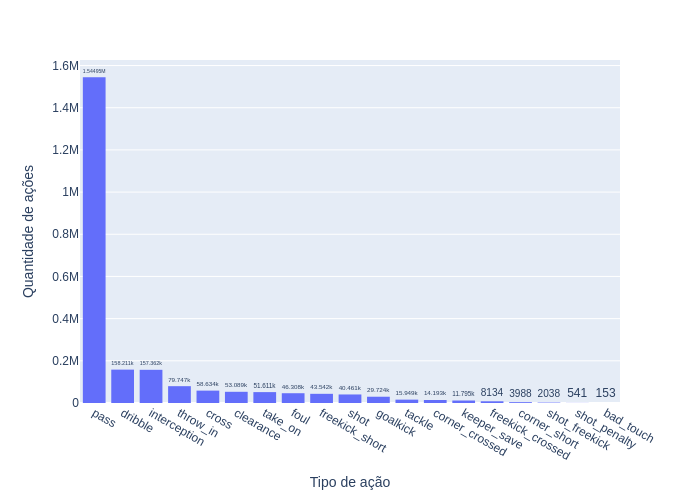
\includegraphics[width=0.8\textwidth]{images/action_distribution.png}
	\caption{Distribuições dos tipos de ação}
	\label{fig:action_distribution}
\end{figure}

\subsection{Distribuição da posição de chutes convertidos em gol}

O mapa de calor abaixo permite que sejam analisadas a distribuição das posições
dos chutes que se converteram em gol
na base de dados.

\begin{figure}[H]
	\centering
	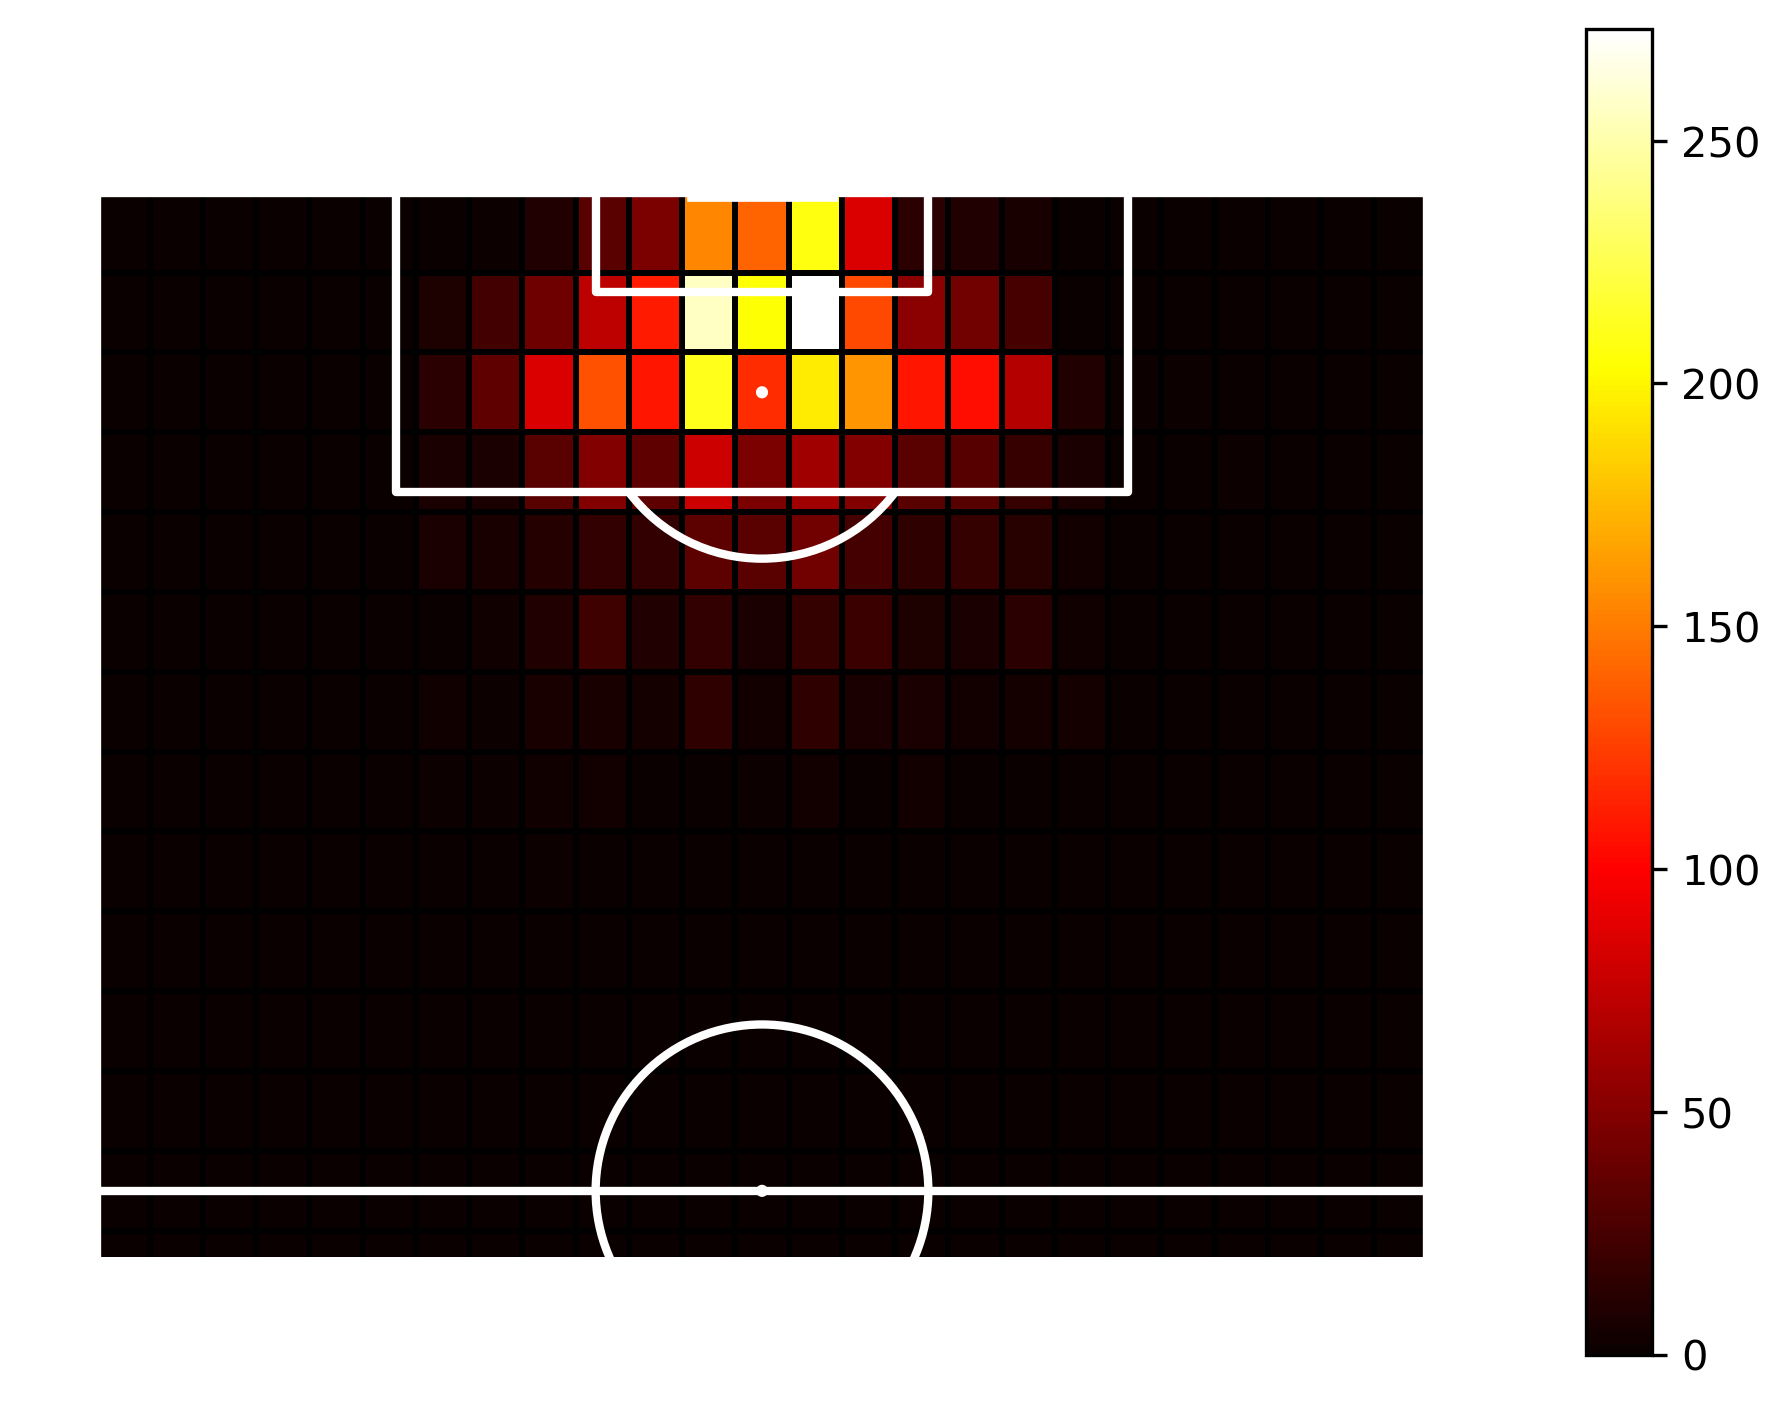
\includegraphics[width=0.5\textwidth]{images/goal_position_heatmap.png}
	\caption{Distribuições dos tipos de ação}
	\label{fig:heatmap_goals}
\end{figure}

\subsection{Distância média entre passes}

O passe é um dos, se não o fundamento mais importante em um esporte coletivo
como o futebol. Uma boa execução desse fundamento por parte dos jogadores
de uma equipe indica um bom controle da posse de bola que está diretamente
conectado com bons resultados \cite{cox2022linhas}. Nesse sentido é
interessante fazer um análise
das distâncias entre os passes
executados por cada equipe.

Em particular, foi coletada a distância entre todos os passes bem sucedidos de
cada equipe e, posteriormente, coletadas estatísticas sobre essas distâncias. A
distância média
entre passes se destacou, uma vez que ela indica como funciona a dinâmica de
troca de passes de uma equipe. Os resultados observados confirmaram suspeitas
prévias acerca do assunto.
Como pode-se notar nas tabelas abaixo, para cada uma das grandes ligas, as
principais equipes, isto é, as equipes com maior grandeza histórica e maior
poderio financeiro figuram como aquelas
que possuem a menor distância média entre passes bem sucedidos. Na Inglaterra,
por exemplo, o Manchester City, equipe comandada pelo espanhol Pep Guardiola,
foi a equipe com a menor média
de distância entre passes. O estilo de jogo de Guardiola é muito focado no
controle da posse de bola e na movimentação dos jogadores para receptar um
passe \cite{terzis2023pep}, então o resultado está dentro do
esperado.

É interessantes notar que os clubes com menor média de distância entre os
passes da temporada 17/18 em cada liga mantiveram posições altas em seus
respectivos campeonatos. O Manchester City e o Paris Saint Germain se sagraram
campeões, enquanto Napoli e Atletico de Madrid ficaram com a segunda colocação.
Na Alemanha, o RB Leipzig ficou com a sexta colocação. Pode-se notar então que
existe uma correlação entre a o desempenho de um time no campeonato com a
distância média entre os passes da equipe.

\begin{table}[H]
	\centering
	\begin{tabular}{|c|c|}
		\hline
		\textbf{Equipe}            & \textbf{Distância média entre
			passes (m)}
		\\ \hline
		Manchester City FC         & 17.208
		\\ \hline
		Arsenal FC                 & 17.729
		\\ \hline
		Manchester United FC       & 17.823
		\\ \hline
		AFC Bournemouth            & 18.417
		\\ \hline
		Tottenham Hotspur FC       & 18.490
		\\ \hline
		Crystal Palace FC          & 18.555
		\\ \hline
		Chelsea FC                 & 18.682
		\\ \hline
		Southampton FC             & 18.801
		\\ \hline
		Liverpool FC               & 18.808
		\\ \hline
		West Ham United FC         & 18.832
		\\ \hline
		Watford FC                 & 18.967
		\\ \hline
		Newcastle United FC        & 18.972
		\\ \hline
		Swansea City AFC           & 19.077
		\\ \hline
		Leicester City FC          & 19.189
		\\ \hline
		Huddersfield Town FC       & 19.215
		\\ \hline
		Stoke City FC              & 19.690
		\\ \hline
		West Bromwich Albion FC    & 19.712
		\\ \hline
		Everton FC                 & 19.785
		\\ \hline
		Brighton \& Hove Albion FC & 19.838
		\\ \hline
		Burnley FC                 & 20.634
		\\ \hline
	\end{tabular}
	\caption{Premier League}
	\label{tab:average_distance_england}
\end{table}


\section{Extração de \textit{Features}}

O foco das análises desse trabalho foram em avaliar eventos que levaram à 
chutes ao gol, na tentativa de tentar entender quais atributos que levam 
(ou não) a pontuar no futebol. Dessa forma, o primeiro pré-processamento foi 
filtrar os eventos de todas as partidas, para capturar as informações só
do evento de chute, além de capturar outras informações.

Mais especialmente, a partir dos atributos listados na \ref{tab:atributosSPADL}, 
realizamos um  pré-processamento para computar métricas adicionais relevantes 
para a nossa análise. Alguns dos valores por sí só já são relevantes e portanto 
foram mantidos, como o nome do jogador, as localizações de onde a ação 
começou (nesse caso, o chute) e qual parte do corpo foi usada. Outras métricas 
foram calculadas, como distância percorrida da bola partindo do chute até o gol, 
e o ângulo do chute relativo ao gol. Já outros atributos foram computadas com base 
nos outros eventos que levaram ao chute: consideramos para a parte de SD desse 
trabalho todos os eventos desde que o time que chutou tem a posse de bola, por 
acreditar que tudo possa fazer parte da estratégia para chegar ao gol (e por ser 
muito difícil definir a partir de qual ponto começou uma jogada que levou ao chute).
Com os eventos que levaram a tentativa de marcar, computamos \textit{features} como 
total de eventos, passes e dribles, velocidade da jogada e duração total, dentre 
outros. Por fim, utilizamos a informação de avaliações (ranking) dos jogadores 
nas partidas para complementar a análise. Todos os atributos utilizados estão 
na tabela \ref{tab:atributosSD}.

\begin{table}[H]
    \centering
    \begin{tabularx}{\textwidth}{|l|X|}
        \hline
        \textbf{Atributo} & \textbf{Descrição} \\
        \hline
        start\_x & A localização x onde a ação começou \\
        \hline
        start\_y & A localização y onde a ação começou \\
        \hline
        num\_events & Contagem total de eventos (ações) na jogada \\
        \hline
        num\_passes & Contagem total de passes na jogada \\
        \hline
        num\_dribles & Contagem total de dribles na jogada \\
        \hline
        play\_duration & Duração total da jogada \\
        \hline
        player\_rank & Ranking do jogador \\
        \hline
        play\_distance & Distância (euclidiana) total percorrida na jogada \\
        \hline
        play\_mean\_distance\_to\_the\_goal & Distância (euclidiana) média de cada jogada até o gol \\
        \hline
        play\_std\_distance\_to\_the\_goal & Desvio padrão da distância (euclidiana) de cada jogada até o gol \\
        \hline
        play\_distance\_towards\_goal & Distância percorrida nas jogadas em direção ao gol (considerando só o eixo x) \\
        \hline
        bodypart\_name & A parte do corpo do jogador usada para a ação \\
        \hline
        ratio\_distance & Razão entre play\_distance e play\_distance\_towards\_goal \\
        \hline
        total\_time\_per\_play & Desvio padrão da distância (euclidiana) de cada jogada até o gol \\
        \hline
        play\_duration & Duração total das jogadas \\
        \hline
        total\_time\_per\_play & Média do tempo por jogada (razão entre play\_duration e num\_events) \\
        \hline
        play\_speed & Razão entre play\_distance e play\_duration \\
        \hline
        play\_speed\_towards\_goal & Razão entre play\_distance\_towards\_goal e play\_duration \\
        \hline
    \end{tabularx}
    \caption{Atributos utilizados na descoberta de subgrupos}
    \label{tab:atributosSD}
\end{table}

\section{Descoberta de Subgrupos}

Os dados disponibilizados pela \textit{Wyscout} possuem diversas granularidades: 
temos 5 ligas de 5 países diferentes, cada uma com suas características, e cada 
uma com seus respectivos times e estilo. Visando avaliar essas diferenças, a 
análise de Descoberta de Subgrupos foi dividida em 3 partes: na primeira, 
avaliamos os grupos descobertos de todo o dataset com os datasets de duas ligas 
expecíficas (da Inglaterra e da Espanha), para ver se encontramos diferenças 
entre uma liga VS toda a "população". Na segunda, escolhemos três times de uma 
mesma liga, um que terminou no topo da tabela, outro no meio e outro que ficou 
em último, para analisar se essa diferença de posição se reflete nos padrões. Por 
fim, avaliamos todo o dataset com duas estratégias diferentes de SD, para avaliar 
redundância e diversidade entre estratégias.

Em todas avaliações foi utilizado a estratégia de \textit{Beam Search} 
do pacote do \textit{pysubgroup}, com profundidade 3, buscando 100 subgrupos com 
largura do Beam de 250. Na terceira, utilizamos o \textit{SSD++} com profundidade 
3, largura do beam de 25 e máximo de regras 20 (o que gerou aproximadamente 100 
resultados, para comparar com a outra abordagem). Também, em todas as etapas 
foram avaliados todos os alvos, sendo se foi realmente gol ou não (binário), o xg 
(binarizado na condição xG >= 0.5), e também a VAEP (numérico).


\section{Mineração de Sequências}

Também foram aplicadas técnicas de mineração de sequências para encontrar
padrões de tipos de ações realizadas antes de um chute ao gol. Para realizar a
mineração de sequências foram usadas algumas técnicas. 

Uma delas foi inspirada em \cite{bunker2021supervised}: o \textit{Safe Pattern
Pruning} (SPP). Usado originalmente no rugby, com resultados promissores,
avaliou-se a viabilidade de aplicar o mesmo algoritmo no contexto do futebol.
Para isso, os dados foram adaptados ao formato de entrada do programa publicado
pelos autores do artigo: cada linha possui um número para indicar a prosperidade
da sequência de ações (1 para resultado promissor e -1 para caso contrário) e
uma sequência de ações propriamente dita.

As sequências de ações são definidas com base na troca de posse de bola, até
ocorrer algum chute ao gol (\textit{shot}). As ações foram definidas como números, conforme a
tabela \ref{tab:id_to_action_map}.

\begin{table}[H]
	\centering
	\begin{tabular}{|c|c|}
		\hline
		\textbf{ID}            & \textbf{Ação}
		\\ \hline
		0 & pass
		\\ \hline
		1 & interception
		\\ \hline
		2 & dribble
		\\ \hline
		3 & take on
		\\ \hline
		4 & tackle
		\\ \hline
		5 & foul
		\\ \hline
		6 & freekick short
		\\ \hline
		7 & cross
		\\ \hline
		\textbf{8} & \textbf{shot}
		\\ \hline
		9 & clearance
		\\ \hline
		10 & throw in
		\\ \hline
		11 & goalkick
		\\ \hline
		12 & corner short
		\\ \hline
		13 & corner crossed
		\\ \hline
		14 & keeper save
		\\ \hline
		15 & freekick crossed
		\\ \hline
		16 & shot freekick
		\\ \hline
		17 & bad touch
		\\ \hline
		18 & shot penalty
		\\ \hline
	\end{tabular}
	\caption{Mapeamento de Ações para IDs}
	\label{tab:id_to_action_map}
\end{table}

Para definir se o resultados das ações foi promissor, foram usadas 3 métricas
distintas: o \textit{xG}, o VAEP e uma classificação binária que indica o
resultado da ação (no caso de um chute ao gol, se a ação marcou um ponto). O
\textit{xG} foi estimado com uso de um \textit{RandomForest}, considerando a
parte do corpo associada ao chute (categoricamente), a distância até o gol e o
ângulo entre o chute e o gol. Já o VAEP foi treinado com um \textit{XGBoost},
discretizando-se com um valor de $P_{scores}$ igual a $\frac{1}{2}$. Ou seja,
apenas chutes cuja probabilidade de marcar foi maior que $\frac{1}{2}$ foram
considerados promissores.

Os parâmetros usados na execução foram: tamanho máximo dos padrões igual a 5,
suporte mínimo igual a 50, multiprocessamento habilitado. Traduzindo-se para as
\textit{flags} utilizadas no programa:

\begin{center}
	\texttt{-L 5 -m 50 -M 1}
\end{center}

Apesar dos bons resultados no rugby em \cite{bunker2021supervised}, as sequências obtidas deixaram a desejar
quanto aplicadas ao futebol, independentemente da métrica usada. Em todos os
casos, as sequências de jogadas obtidas eram muito redundantes, continham passes
(0) em excesso ou não eram muito surpreendentes. Por exemplo, uma sequência de
passes seguida por um cruzamento (7). Os arquivos de saída gerados podem ser
obtidos
\href{https://github.com/lframosferreira/projeto-ad/blob/main/results/supervised-sequential-pattern-rugby/results_xg.csv}{aqui}
para o \textit{xG},
\href{https://github.com/lframosferreira/projeto-ad/blob/main/results/supervised-sequential-pattern-rugby/results_binary.csv}{aqui}
para o binário e
\href{https://github.com/lframosferreira/projeto-ad/blob/main/results/supervised-sequential-pattern-rugby/results_vaep.csv}{aqui}
para o VAEP.

Uma possível explicação para os resultados encontrados é o fato de o futebol ser
um esporte muito dinâmico e que, por essa natureza, exigiria outra abordagem
para discretização dos dados, para além das sequências de ações. De fato, muitos
gols são (e não são) marcados a partir de uma sequência de passes, por exemplo.
Desse modo, uma abordagem que consiga mapear o campo de maneira mais sutil é
necessária para que se possa realizar uma mineração de sequências usando o
algoritmo proposto por \cite{bunker2021supervised}.

\section{Resultados}

\subsection{Avaliação geral}

Na tabela \ref{tab:resultMetricas} são apresentados os resultados das métricas obtidas 
em cada uma das etapas, considerando cada um dos algoritmos, dataset utilizado e os diferentes 
alvos. Podemos ver que, de maneira geral, o \textit{expected Goals} (xG) foi o que desempenhou 
pior dos três alvos, com tendências de WRAcc mais baixas, e coberturas também. O VAEP e o resultado 
real (se foi gol ou não) tiveram comportamento bem semelhante, sendo mais altos ou baixo juntos 
(indicando uma certa correlação). Por fim, apesar de algumas variações nos resultados, o SSD++ 
demonstrou ser uma estratégia bem  mais abrangente no quesito de cobertura, ao custo de um WRAcc 
menor. Esse resultado condiz com os resultados do artigo \ref{covid}, onde isso também foi percebido. 
Vale ressaltar que apesar dos testes envolvendo Beam Search terem coberturas altas (pois foram 
gerados 100 subgrupos), os resultados são bem redundantes (veja subseção 5.4).

\begin{table}[H]
	\centering
	\begin{tabular}{|l|l|l|l|l|}
		\hline
		\textbf{Algoritmo} & \textbf{Dado} &  \textbf{Target} & 
		\textbf{WRAcc do melhor} & \textbf{Cobertura Total}
		\\
		\hline
		Beam Search & Todo dataset & Gol & 0.0312 & 0.5099 
		\\
		\hline
		Beam Search & Todo dataset & xG & 0.0187 & 0.5046 
		\\
		\hline
		Beam Search & Todo dataset & VAEP & 0.0307 & 0.5099 
		\\
		\hline
		Beam Search & Inglaterra & Gol & 0.03192 & 0.4980 
		\\
		\hline
		Beam Search & Inglaterra & xG & 0.0203 & 0.4933 
		\\
		\hline
		Beam Search & Inglaterra & VAEP & 0.0317 & 0.4977
		\\
		\hline
		Beam Search & Espanha & Gol & 0.0307 & 0.5110 
		\\
		\hline
		Beam Search & Espanha & xG & 0.0195 & 0.3983 
		\\
		\hline
		Beam Search & Espanha & VAEP & 0.0304 & 0.5120 
		\\
		\hline
		Beam Search & Man City & Gol & 0.0483 & 0.5721 
		\\
		\hline
		Beam Search & Man City & xG & 0.0303 & 0.4959 
		\\
		\hline
		Beam Search & Man City & VAEP & 0.0487 & 0.5656 
		\\
		\hline
		Beam Search & Newcastle & Gol & 0.0405 & 0.6561 
		\\
		\hline
		Beam Search & Newcastle & xG & 0.0247 & 0.3878 
		\\
		\hline
		Beam Search & Newcastle & VAEP & 0.0420 & 0.6561 
		\\
		\hline
		Beam Search & West Bromwich & Gol & 0.0293 & 0.5499 
		\\
		\hline
		Beam Search & West Bromwich & xG & 0.0307 & 0.3989 
		\\
		\hline
		Beam Search & West Bromwich & VAEP & 0.0287 & 0.5254 
		\\
		\hline
		SSD++ & Todo Dataset & Gol & 0.0164 & 0.7818 
		\\
		\hline
		SSD++ & Todo Dataset & xG & 0.0117 & 0.9956
		\\
		\hline
		SSD++ & Todo Dataset & VAEP & 0.0269 & 0.9177
		\\
		\hline
	\end{tabular}
	\caption{Descrição dos dados no formato SPADL}
	\label{tab:resultMetricas}
\end{table}


\subsection{Avaliação entre ligas}

Na tabela \ref{tab:resultsSD} temos alguns subgrupos de cada uma das análises dos datasets, 
considerando os três diferentes alvos.

\begin{table}[H]
    \centering
    \begin{tabularx}{\textwidth}{|l|l|X|}
        \hline
        \textbf{Dataset} & \textbf{Target} & \textbf{Subgrupo} \\
        \hline
        Todo dataset & Gol & $ \text{shot\_angle\_from\_goal} \geq 0.60 \ \text{AND} \ \text{shot\_distance\_from\_goal} < 11.26 $ \\
        \hline
        Todo dataset & xG & $ \text{shot\_angle\_from\_goal} \geq 0.60 \ \text{AND} \ \text{shot\_distance\_from\_goal} < 11.26 \ \text{AND} \ \text{start\_x} \geq 96.60 $ \\
        \hline
        Todo dataset & VAEP & $ \text{num\_dribbles} : [0:1[ \ \text{AND} \ \text{shot\_angle\_from\_goal} \geq 0.60 \ \text{AND} \ \text{shot\_distance\_from\_goal} < 11.26 $ \\
        \hline
        Inglaterra & Gol & $ \text{shot\_angle\_from\_goal} \geq 0.61 \ \text{AND} \ \text{shot\_distance\_from\_goal} < 11.26 $ \\
        \hline
        Inglaterra & xG & $ \text{num\_dribbles} : [0:1[ \ \text{AND} \ \text{shot\_distance\_from\_goal} < 11.26 \ \text{AND} \ \text{start\_x} \geq 96.60 $ \\
        \hline
        Inglaterra & VAEP & $ \text{play\_duration} < 1.39 \ \text{AND} \ \text{shot\_distance\_from\_goal} < 11.26 \ \text{AND} \ \text{total\_time\_per\_play} < 0.65 $ \\
        \hline
        Espanha & Gol & $ \text{shot\_angle\_from\_goal} \geq 0.61 \ \text{AND} \ \text{shot\_distance\_from\_goal} < 11.04 \ \text{AND} \ \text{start\_x} \geq 96.60 $ \\
        \hline
        Espanha & xG & $ \text{shot\_angle\_from\_goal} \geq 0.61 $ \\
        \hline
        Espanha & VAEP & $ \text{play\_distance\_towards\_goal} : [0.0:7.35[ \ \text{AND} \ \text{ratio\_distance} : [0.0:0.12[ \ \text{AND} \ \text{shot\_distance\_from\_goal} < 11.04 $ \\
        \hline
    \end{tabularx}
    \caption{Resultados para diferentes alvos}
    \label{tab:resultsSD}
\end{table}

Os subgrupos foram escolhidos dos top-10 considerando WRAcc, com exceção dos do alvo VAEP para os 
datasets de ligas isoladas, para ter maior variedade. O mais perceptível é a redundância dos subgrupos, 
onde todos são arranjos de cinco ou seis atributos principais. Contudo, podemos perceber pequenas 
diferenças, como nas distâncias e ângulos para o chute. A medida que descemos as listas dos subgrupos 
obtidos também temos mais variações, aparecendo features como ranking do jogador, quantidade de passes, 
dentre outras. Outro fato interessante é de que as métricas concordam entre si, nos subgrupos e nos valores.

\subsection{Avaliação entre times}

\subsection{Avaliação entre algoritmos de SD}

\section{Conclusão}

fefre

\newpage
\bibliographystyle{plain}
\renewcommand{\refname}{Referências Bibliográficas}
\addcontentsline{toc}{section}{Referências Bibliográficas}
\bibliography{sample}
\nocite{*}

\end{document}
